\documentclass[12pt, a4paper]{report}

% === Package start ===
\usepackage{fontspec} % 加這個就可以設定字體
\usepackage{xeCJK} % 讓中英文字體分開設置
\usepackage{graphicx} % 引入圖片
\usepackage{indentfirst}
\usepackage{hyperref}
\usepackage{listings} % for code listing
\usepackage{xcolor} % for code listing color settings
\usepackage{url}
% === Package end ===

\setcounter{secnumdepth}{4}
\setcounter{tocdepth}{4}
\usepackage{float}
\setCJKmainfont[Path=fonts/]{DFKai-SB.ttf}
\XeTeXlinebreaklocale "zh" % Defines how to break lines for multilingual text
\XeTeXlinebreakskip = 0pt plus 1pt % Inter-character linebreak stretch
\graphicspath{{images/}, {images/NN_img/}}
\setlength{\parindent}{2em}

\hypersetup{
    colorlinks=true,
    linkcolor=black, % Make TOC remain black
    urlcolor=blue,
}

% code listing settings
\definecolor{codegreen}{rgb}{0,0.6,0}
\definecolor{codegray}{rgb}{0.5,0.5,0.5}
\definecolor{codepurple}{rgb}{0.58,0,0.82}
\definecolor{backcolour}{rgb}{0.95,0.95,0.92}
\lstdefinestyle{mystyle}{
    backgroundcolor=\color{backcolour},   
    commentstyle=\color{codegreen},
    keywordstyle=\color{magenta},
    numberstyle=\tiny\color{codegray},
    stringstyle=\color{codepurple},
    basicstyle=\ttfamily\footnotesize,
    breakatwhitespace=false,         
    breaklines=true,                 
    captionpos=b,                    
    keepspaces=true,                 
    numbers=none,                    
    numbersep=5pt,                  
    showspaces=false,                
    showstringspaces=false,
    showtabs=false,                  
    tabsize=2
}
\lstset{style=mystyle}

% === Content start from here ===
\begin{document}

\begin{titlepage}
    \linespread{2} %兩倍行距
    \centering
    \Large 國立台灣海洋大學資訊工程學系專題報告\\
    \LARGE dARt \\
    \ \\
    
\includegraphics[width=3cm]{NTOU-school-badge}\\
   
    \ \\
    \linespread{1}
    \begin{table}[h]
        \large
        \centering
        \begin{tabular}{lll}
            00757303 CSE 5A 李 萱 \\
            00668108 CSE 4A 羅 捷 \\
            00757202 CSE 4A 洪晟洋 \\
            0066c027 CSE 4A 魏資碩 \\
        \end{tabular}
    \end{table}

    \large \hspace{-1cm} 報告編號: NTOUCSE 110學年度-指導老師編號-競賽組第 1 組 \\
    \large 指導教授:張欽圳老師\ \\
    \vspace{3cm}
    \large 中華民國 109 年 XX 月 XX 日

\end{titlepage}

\begin{large}
\centering 專題分工及貢獻度說明
\end{large}

\begin{table}[h]
\begin{tabular}{|l|l|l|l|}
\hline
編號 & 姓名  & 主要工作內容     & 專題貢獻度(100\%) \\\hline
1  & 羅捷  & Android 端 &        35\%      \\\hline
2  & 洪晟洋 &  物理運算  &      20\%        \\\hline
3  & 李萱  & 前後端整合、網路連接 &    20\%          \\\hline
4  & 魏資碩 & 後端神經網路訓練、設計及優化 &  25\%     \\\hline     
\end{tabular}
\end{table}


%==================
% 專案管理系統截圖
%==================



\tableofcontents % Compile twice to correctly show
\listoffigures
\listoftables


% === Chapter ===
\chapter{介紹}
\section{研究目的與動機}

    研究目的

\section{系統簡介(遊戲說明、流程圖、多人運作)}

    系統簡介(遊戲說明、流程圖、多人運作)

\section{系統架構}

    系統架構


% === Chapter ===
\chapter{前端架構}
\section{技術介紹}

前端-在此為 Android 手機-負責了 AR 場景的繪製。這部分藉助了由 Google 所提供的 \href{https://developers.google.com/ar}{ARCore} ,對圖 \ref{fig:標定物} 進行姿態估計與使用 OpenGL ES 繪製 3D 物件於場景中。

\begin{figure}[h]
    \centering
    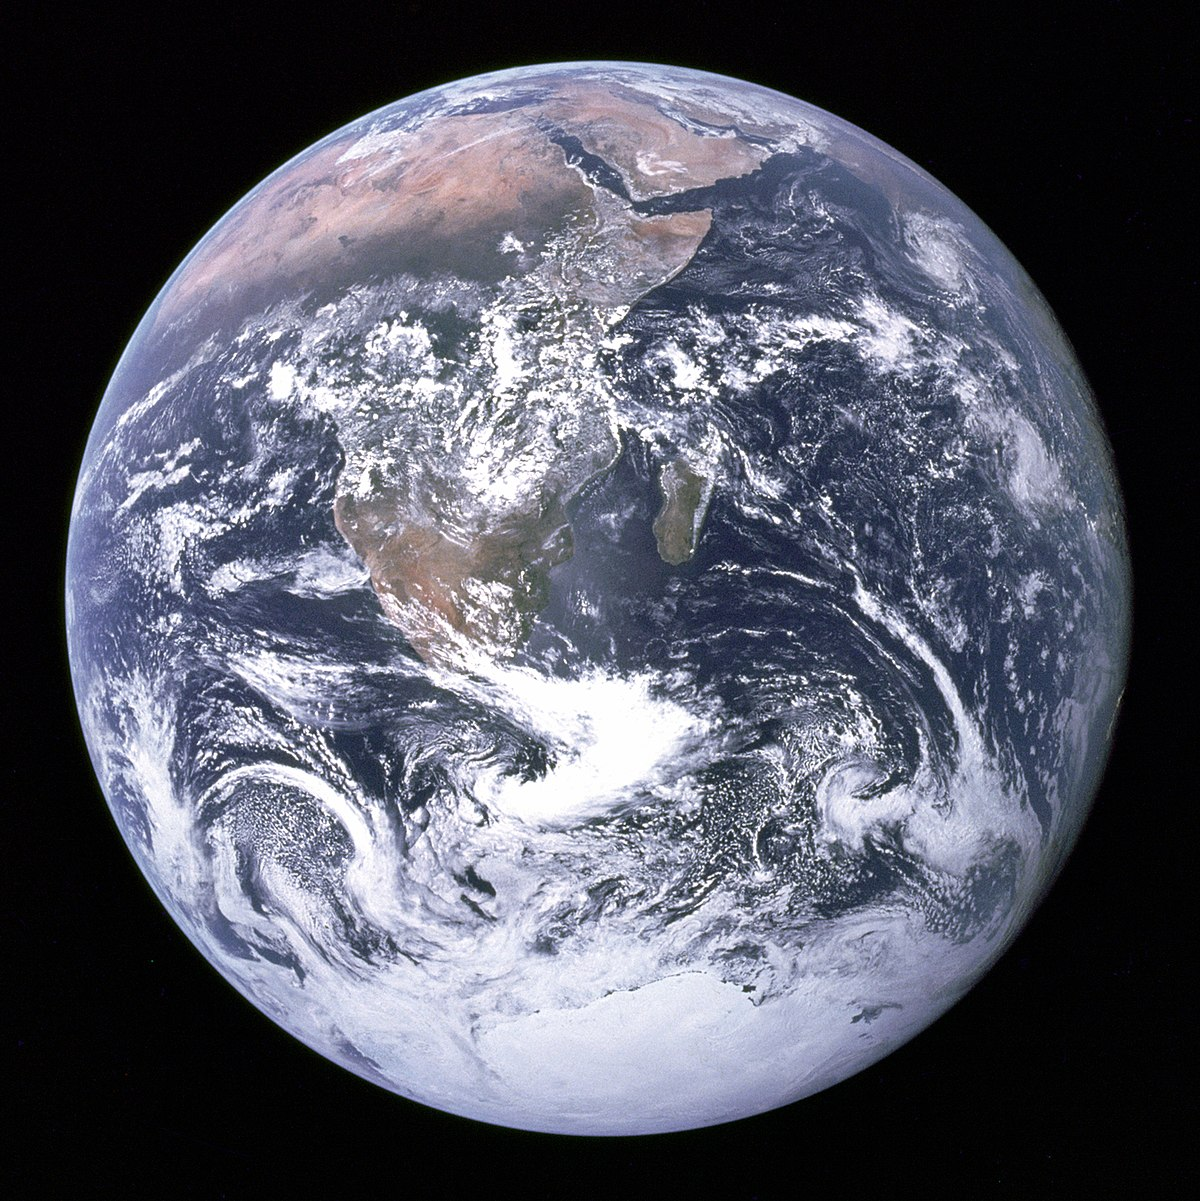
\includegraphics[width=3cm]{mark.jpg}
    \caption{標定物}
    \label{fig:標定物}
\end{figure}

\section{技術說明與實作}
\subsection{ARCore 姿態估計}
\subsubsection{安裝}

欲使用 ARCore 必須先安裝 Google 所提供的應用程式,該應用程式可以在 \href{https://play.google.com/store/apps/details?id=com.google.ar.core}{Google Play} \footnote{\url{https://play.google.com/store/apps/details?id=com.google.ar.core}} 上找到。須注意並非所有 Android 裝置都支援這個應用程式,支援的裝置列表可以在\href{https://developers.google.com/ar/discover/supported-devices#google_play_device}{此處}查詢。

\subsubsection{準備、初始化}

在安裝後需要撰寫一系列繁雜且固定的初始化流程,才能在執行期安全地取得讓我們能夠使用 ARCore 的物件-com.google.ar.core.Session-這一系列的繁雜任務不多做贅述,可以於\href{https://developers.google.com/ar/develop/java/enable-arcore}{此處}查看。

\subsubsection{標定物設定}

為了使標定物能夠被 ARCore 偵測,使用了 \href{https://developers.google.com/ar/develop/java/augmented-images}{Augmented Images} 相關的 API。需要先將影像加入 \href{https://developers.google.com/ar/reference/java/com/google/ar/core/AugmentedImageDatabase}{AugmentedImageDatabase},之後將該物件交給 \href{https://developers.google.com/ar/reference/java/com/google/ar/core/Session}{Session}。具體有二種做法。

於執行時將圖片動態載入 AugmentedImageDatabase:

\begin{lstlisting}[language=Java, caption=動態載入圖片]
InputStream is = getAssets().open("image.png")
Bitmap augmentedImageBitmap = BitmapFactory.decodeStream(is)

AugmentedImageDatabase augmentedImageDatabase;
augmentedImageDatabase = new AugmentedImageDatabase(session);
augmentedImageDatabase.addImage("image", 
                                augmentedImageBitmap,
                                /*widthInMeters = */0.25f);

Config config = new Config(session);
config.setAugmentedImageDatabase(augmentedImageDatabase);
session.configure(config);
\end{lstlisting}

或是預先使用 \href{https://developers.google.com/ar/develop/java/augmented-images/arcoreimg}{arcoreimg tool} 將圖片(可多張)打包成 AugmentedImageDatabase 可讀取的 *.imgdb 檔案

\begin{lstlisting}[language=bash, caption=使用 arcoreimg tool 將圖片打包]
arcoreimg.exe build-db --input_image_list_path=/path/to/image_list_file.txt --output_db_path=/path/to/myimages.imgdb
\end{lstlisting}

image\_list\_file.txt 格式為:以 | 分隔,順序為圖片名稱、圖片位置、圖片物理寬度(公尺,非必要,有助於 ARCore 偵測圖片)。

\begin{lstlisting}[caption=image\_list\_file.txt 範例]
mouse|path/to/mouse.png|0.1
little dog|/path/to/dog.jpg
\end{lstlisting}

之後便可將 myimages.imgdb 交給 Session

\begin{lstlisting}[language=Java, caption=將 myimages.imgdb 交給 Session]
AugmentedImageDatabase augmentedImageDatabase;
InputStream is = getAssets().open("myimages.imgdb")
augmentedImageDatabase = AugmentedImageDatabase.deserialize(session, is);

Config config = new Config(session);
config.setAugmentedImageDatabase(augmentedImageDatabase);
session.configure(config);
\end{lstlisting}

\subsubsection{偵測標定物}
將 AugmentedImageDatabase 透過 Config 設定給 Session 後,便可透過 \lstinline{session.update()} 更新 Augmented Image 的追蹤情形。

\begin{lstlisting}[language=Java, caption=取得影像追蹤狀態]
Frame frame = session.update();
Collection<AugmentedImage> updatedAugmentedImages = frame.getUpdatedTrackables(AugmentedImage.class);

for (AugmentedImage augmentedImage : updatedAugmentedImages) {
    switch (augmentedImage.getTrackingState()) {
        case PAUSED:
            // When an image is in PAUSED state, but the camera is not PAUSED, it has been detected, but not yet tracked.
            break;

        case TRACKING:
            // The Trackable is currently tracked and its pose is current.
            break;

        case STOPPED:
            // ARCore has stopped tracking this Trackable and will never resume tracking it.
            break;

        default:
            break;
}
\end{lstlisting}

\subsubsection{取得標定物姿態}

在 Tracking 狀態下,可透過 \lstinline{augmentedImage.getCenterPose()} 取得 Augmented Image 在世界坐標系(該坐標系由 ARCore 管理)的姿態(未 Tracking 時會是上一次 Tracking 的最後位置),該姿態 +X 軸從影像左側指向右側, +Z 軸從影像上側指向下側,+Y 軸指出該平面。

\subsection{OpenGL 物件位置與實景貼合}

透過 OpenGL 繪製物件需透過三個 Matrix 完成座標點的轉換:分別為 Projection, View, Model

\subsubsection{Model Matrix}
將位於 Model coordinate 的座標點轉移至 World coordinate

\subsubsection{View}
將位於 World coordinate 的座標點轉移至 Camera coordinate

\subsubsection{Projection}
將位於 Camera coordinate 的座標點轉移至 Clip coordinate。

\begin{center}
    $
        coordinate\_in\_clip = Projection\_Matrix \times View\_Matrix \times Model\_Matrix \times model\_coordinate
    $
\end{center}

這些矩陣皆可透過 ARCore 取得,僅需注意其順序為 Column-major。

\subsubsection{取得 Model Matrix}

Model matrix 可以由藉由追蹤中物件取得,例如想取得將 3D Model 轉移至標定物姿態的矩陣。

\begin{lstlisting}[language=Java, caption=將 3D model 的座標空間轉移至以標定物為準的空間]
Frame frame = session.update();
Collection<AugmentedImage> updatedAugmentedImages = frame.getUpdatedTrackables(AugmentedImage.class);

// Assume only one image
AugmentedImage augmentedImage = updatedAugmentedImages.iterator().next();

float[] modelMatrix = new float[16];
switch (augmentedImage.getTrackingState()) {
    case TRACKING:
        augmentedImage.getCenterPose().toMatrix(modelMatrix, /*offset = */ 0);
        break;

    default:
        break;
}
\end{lstlisting}

\subsubsection{取得 View Matrix}

相機坐標系的管理由 ARCore 掌握,若想取得 View Matrix。

\begin{lstlisting}[language=Java, caption=取得 View Matrix]
Frame frame = session.update();
Camera camera = frame.getCamera();

float[] viewMatrix = new float[16];
camera.getViewMatrix(viewMatrix, /*offset = */ 0);
\end{lstlisting}

\subsubsection{取得 Projection Matrix}

投影矩陣做法也類似。

\begin{lstlisting}[language=Java, caption=取得 Projection Matrix]
float[] projMatrix = new float[16];
camera.getProjectionMatrix(projMatrix,
/*offset = */ 0, /*near clipping plane = */ 0.01f, /*far clipping plane = */ 15.0f);
\end{lstlisting}


% === Chapter ===
\chapter{前後端傳輸}
\section{技術介紹}
前後端的傳輸主要使用UDP Socket來做傳輸,主要功能如下:
\begin{itemize}
\item 將手機後相機影像傳送至伺服器,交由神經網路模組辨識手勢。
\item 多人遊玩 - 玩家之間的遊戲資料傳遞。 
若使用者有中靶,傳遞飛鏢的Pose(Translation \& Quaternion)參數至伺服器,在將這些資料傳遞至其他使用者讓其他使用者能看到彼此發射的飛鏢。
\end{itemize}
\subsection{傳輸流程說明}
\begin{figure}[h]
    \centering	
    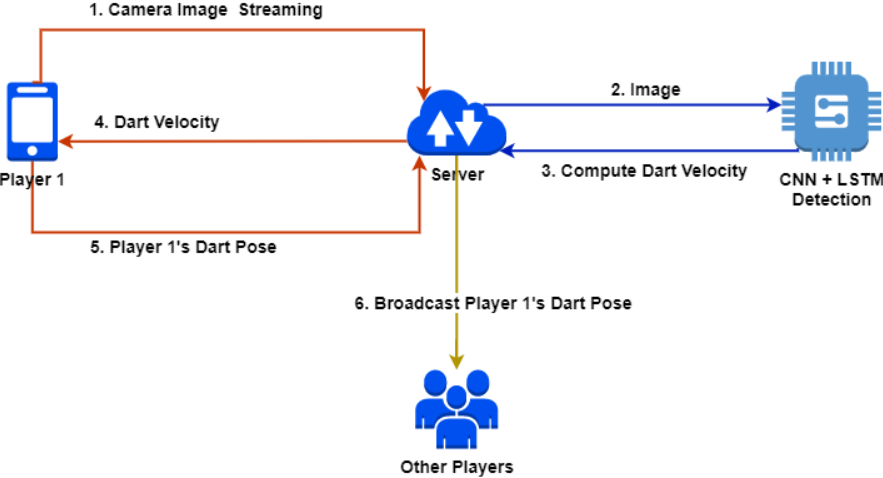
\includegraphics[width=\testwidth]{flow.png}
    \caption{流程圖}
    \label{fig:flow}
\end{figure}
\begin{enumerate}
\item 手機後相機影像擷取,傳輸至伺服器。
\item 伺服器解壓影像,將影像傳送至神經網路模組。
\item 神經網路模組辨識飛鏢速度 。
\item 飛鏢速度由伺服器端傳送至手機端。
\item 若玩家中靶,則將飛鏢之位置(Pose)傳送至伺服器。
\item 伺服器傳送中靶位置給其他使用者。
\end{enumerate}

影像以及遊戲資料個別使用一個Socket,目的是將資料分流,另外也能夠在伺服器端做multi-process的處裡,加快處裡速度。
\subsection{手機端實作}
\subsubsection{手機後相機影像的擷取}
1. 在onDrawFrame()裡,在camera preview image render到 GL surface之後,將GL的surfaceView儲存到buffer,轉換為Bitmap。

2. 每個pixel需儲存R,G,B,A這四個資料,因此 buffer allocate memory = surfaceView’s width * height * 4 bytes。

3. 在create完buffer後,需呼叫rewind(),將buffer的position設為0,將讀取的資料位置從0開始。\href{可於此處}{https://stevenitlife.blogspot.com/2015/01/java-nio-socket-bytebuffer-method.html} 了解相關buffer使用方法。

\begin{lstlisting}[language=Java, caption=手機後相機影像擷取]
// Create buffer: allocate memory( 1 pixel = 4 bytes(R, G, B, A))
ByteBuffer bf = ByteBuffer.allocateDirect(surfaceView.getWidth() * surfaceView.getHeight() * 4);
// Using nativeOrder to store in buffer (other option: Big Endian / Little Endian)
bf.order(ByteOrder.nativeOrder());

// Camera view to buffer
GLES10.glReadPixels(0, 0, surfaceView.getWidth(), surfaceView.getHeight(),
        GLES30.GL_RGBA, GLES30.GL_UNSIGNED_BYTE, bf);
// Create bitmap
Bitmap bmp = Bitmap.createBitmap(surfaceView.getWidth(), surfaceView.getHeight(), Bitmap.Config.ARGB_8888);
bf.rewind();
// Copy buffer data to bitmap
bmp.copyPixelsFromBuffer(bf);

conn.mBackgroundHandler.post(conn.new SendImageData(bmp));
\end{lstlisting}

\subsubsection{傳輸影像至伺服器端}
1. Android的操作,只要超過5秒沒回應(或OnCreate()超過10秒),程式就會被當作無回應,而系統會丟出ANR(Application No Response Exception)。所以,比較耗時費工的動作,都應該考慮用背景作業的方式來完成(另外這些background thread不能包含UI的處理),此處傳輸即用Background Thread做處理。

2. 使用UDP socket傳輸,和TCP不同的是,每次UDP送出的封包都需指定送出的對象(connectionless protocol),不須事先建立連線,且沒有重送封包的機制,因此我們在此專題需要即時上的應用時,選用此技術。

3. 在傳輸Bitmap時,需要轉為byteArray,另外,將Bitmap resize 原大小的1/100,目的想將資料傳輸量盡量變小,降低延遲。

\begin{lstlisting}[language=Java, caption=傳輸影像至伺服器端]
public class SendImageData implements Runnable {
        private Bitmap mBitMap;
        private Bitmap resizeBitMap;
        private byte[] data = null;

        public SendImageData(Bitmap bmp) {
            mBitMap = bmp;
            resizeBitMap = Bitmap.createScaledBitmap(mBitMap, mBitMap.getWidth() / 10, mBitMap.getHeight() / 10, true);
        }

        @Override
        public void run() {
            try {
                if (serverAddr == null) {
                    serverAddr = InetAddress.getByName("140.121.196.201");
                }
                if (socket == null) {
                    socket = new DatagramSocket();
                }

                ByteArrayOutputStream byteStream = new ByteArrayOutputStream();
                resizeBitMap.compress(Bitmap.CompressFormat.JPEG, 80, byteStream);
                data = byteStream.toByteArray();
                try {
                    DatagramPacket packet = new DatagramPacket(data, data.length, serverAddr, 5000);
                    Log.i("data length", String.valueOf(data.length));
                    socket.send(packet);
                } catch (Exception e) {
                    System.out.println("Error 1:" + e.toString());
                }
            } catch (Exception e) {
                System.out.println("Error 2:" + e.toString());
                socket.close();
            }
            mBitMap.recycle();
        }
    }
\end{lstlisting}
\subsection{系統延遲實驗}
\subsubsection{實驗說明}
為達良好之遊戲體驗,故衡量玩家從傳輸影像到拿到回傳參數的時間。而為將各個變因獨立衡量,將分析延遲如下圖所示:

\begin{figure}[h]
    \centering	
    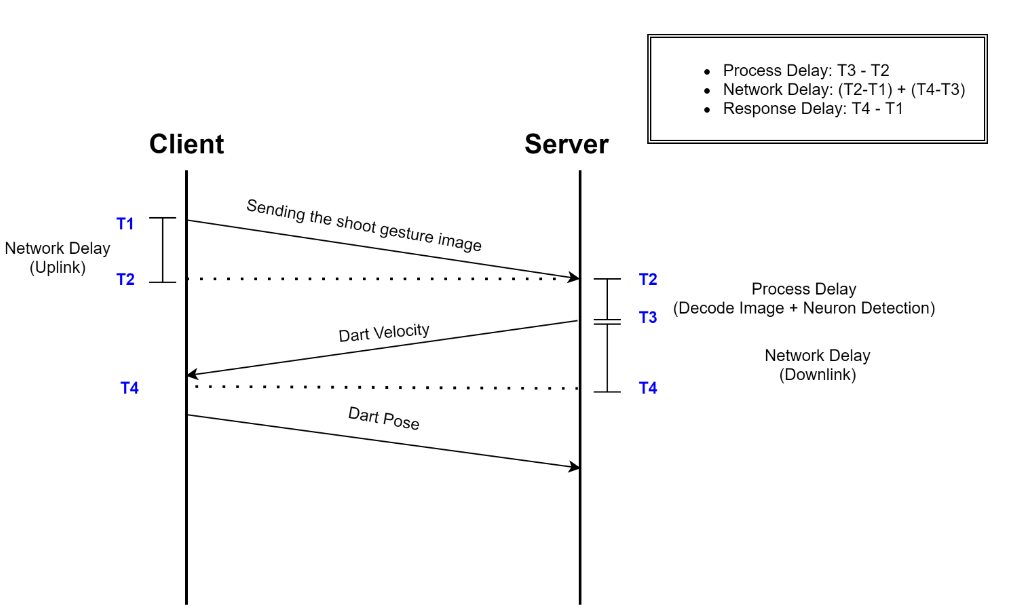
\includegraphics[width=\testwidth]{latency.png}
    \caption{解構響應延遲}
    \label{fig:decomposition of response delay}
\end{figure}

\begin{itemize}
\item Response Delay:
總延遲,玩家由送出手機後相機影像,至拿到飛鏢初速之時間。根據上圖所示,計算方式為T4 - T1。
\item Process Delay:
伺服器端處裡時間,包含影像解碼、神經網路辨識,到送出飛鏢速度的這段時間。根據上圖所示,計算方式為T3 - T2。
\item Network Delay:
網路延遲時間,分為uplink、downlink delay。根據上圖所示,計算方式為(T2-T1) + (T4 - T3)。
\end{itemize}
\subsubsection{系統延遲實驗結果\&分析}
Network Delay主要以ping server來分析,而經過約15次的測試下,平均Network Delay介於40 - 60 ms之間。

Process Delay 則以伺服器接收到影像的時間搓記,與送出封包的時間搓記,來計算其時間差,實驗兩次,每次計算約80 - 100張影像,平均值為7.02 ms 以及7.72ms,Process Delay結果如下圖所示。

\begin{figure}[h]
    \centering	
    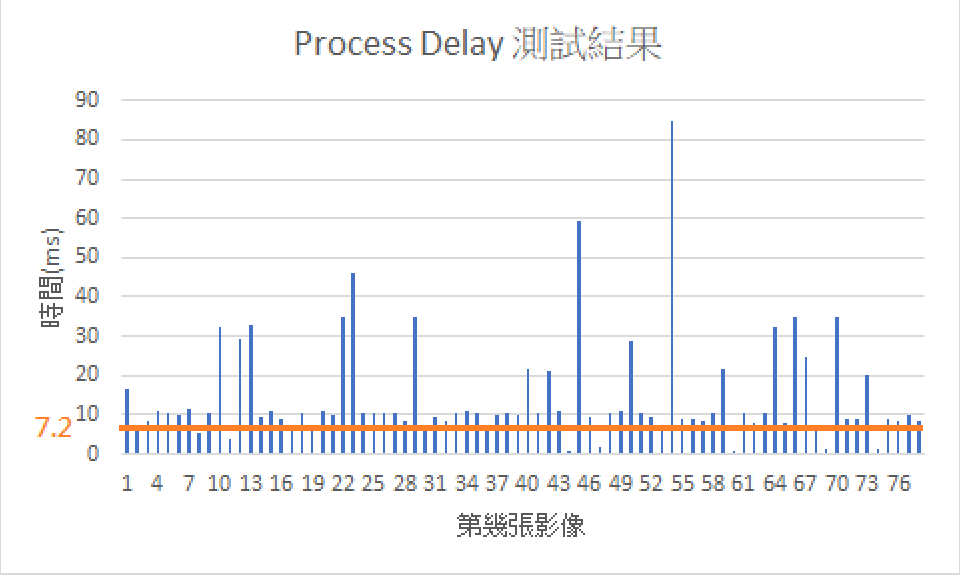
\includegraphics[width=\testwidth]{process_delay.png}
    \caption{實驗一之結果}
    \label{fig:Process delay bar chart}
\end{figure}

結果顯示,Response Delay介於47.02 - 60.72 ms之間,故在發射飛鏢手勢時,不會感到明顯延遲。



% === Chapter ===
\chapter{後端架構}
\section{技術介紹}

    技術介紹

\section{技術說明與實作}
後端 - 以下列出主要兩大功能,並簡述其技術:
\begin{itemize}
\item 由手機端接收到的影像,計算使用者手勢發射飛標之速度。
手機與伺服器之間使用UDP Socket 溝通將手機後相機影像至伺服器,交由神經網路模組( SRCNN + LSTM )並搭載GForce 1080ti GPU加速計算出結果,再回傳至手機。
\item 多人遊玩 - 玩家之間的遊戲資料傳遞。
若使用者有中靶,傳遞飛鏢的Pose(Translation & Quaternion)參數至伺服器,在將這些資料傳遞至其他使用者讓其他使用者能看到彼此發射的飛鏢。
\end{itemize}

伺服器的使用Linux Server 18.04,並使用tmux,方便組態多種操作環境以及背景Session執行。

% 補充1. 神經網路training的環境 2. 神經網路在伺服器上的環境

\subsection{網路端實作}
\subsubsection{手機後相機影像的擷取}
\subsubsection{說明}
1. 在onDrawFrame()裡,在camera preview image render到 GL surface之後,將GL的surfaceView儲存到buffer,轉換為Bitmap。

2. 每個pixel需儲存R,G,B,A這四個資料,因此 buffer allocate memory = surfaceView’s width * height * 4 bytes。

3. 在create完buffer後,需呼叫rewind(),將buffer的position設為0,將讀取的資料位置從0開始。\href{可於此處}{https://stevenitlife.blogspot.com/2015/01/java-nio-socket-bytebuffer-method.html} 了解相關buffer使用方法。

\begin{lstlisting}[language=Java, caption=手機後相機影像擷取]
// Create buffer: allocate memory( 1 pixel = 4 bytes(R, G, B, A))
ByteBuffer bf = ByteBuffer.allocateDirect(surfaceView.getWidth() * surfaceView.getHeight() * 4);
// Using nativeOrder to store in buffer (other option: Big Endian / Little Endian)
bf.order(ByteOrder.nativeOrder());

// Camera view to buffer
GLES10.glReadPixels(0, 0, surfaceView.getWidth(), surfaceView.getHeight(),
        GLES30.GL_RGBA, GLES30.GL_UNSIGNED_BYTE, bf);
// Create bitmap
Bitmap bmp = Bitmap.createBitmap(surfaceView.getWidth(), surfaceView.getHeight(), Bitmap.Config.ARGB_8888);
bf.rewind();
// Copy buffer data to bitmap
bmp.copyPixelsFromBuffer(bf);

conn.mBackgroundHandler.post(conn.new SendImageData(bmp));
\end{lstlisting}

\subsubsection{傳輸影像至伺服器端}
1. Android的操作,只要超過5秒沒回應(或OnCreate()超過10秒),程式就會被當作無回應,而系統會丟出ANR(Application No Response Exception)。所以,比較耗時費工的動作,都應該考慮用背景作業的方式來完成(另外這些background thread不能包含UI的處理),此處傳輸即用Background Thread做處理。

2. 使用UDP socket傳輸,和TCP不同的是,每次UDP送出的封包都需指定送出的對象(connectionless protocol),不須事先建立連線,且沒有重送封包的機制,因此我們在此專題需要即時上的應用時,選用此技術。

3. 在傳輸Bitmap時,需要轉為byteArray,另外,將Bitmap resize 原大小的1/100,目的想將資料傳輸量盡量變小,降低延遲。

\begin{lstlisting}[language=Java, caption=傳輸影像至伺服器端]
public class SendImageData implements Runnable {
        private Bitmap mBitMap;
        private Bitmap resizeBitMap;
        private byte[] data = null;

        public SendImageData(Bitmap bmp) {
            mBitMap = bmp;
            resizeBitMap = Bitmap.createScaledBitmap(mBitMap, mBitMap.getWidth() / 10, mBitMap.getHeight() / 10, true);
        }

        @Override
        public void run() {
            try {
                if (serverAddr == null) {
                    serverAddr = InetAddress.getByName("140.121.196.201");
                }
                if (socket == null) {
                    socket = new DatagramSocket();
                }

                ByteArrayOutputStream byteStream = new ByteArrayOutputStream();
                resizeBitMap.compress(Bitmap.CompressFormat.JPEG, 80, byteStream);
                data = byteStream.toByteArray();
                try {
                    DatagramPacket packet = new DatagramPacket(data, data.length, serverAddr, 5000);
                    Log.i("data length", String.valueOf(data.length));
                    socket.send(packet);
                } catch (Exception e) {
                    System.out.println("Error 1:" + e.toString());
                }
            } catch (Exception e) {
                System.out.println("Error 2:" + e.toString());
                socket.close();
            }
            mBitMap.recycle();
        }
    }
\end{lstlisting}
\subsection{後端神經網路系統架構圖}

主要分為四部份,分別為SRCNN、手部物件辨識、LSTM以及特殊函數轉換.。首先利用SRCNN將手機傳來的照片做高解析化,使手部物件辨識模型辨識率提高。在將手部辨識結果的機率分布傳至LSTM做發射手勢辨識。最後通過函數轉換後回傳發射參數,流程圖請見Figure 3.1。

\begin{figure}[H]
    \centering
    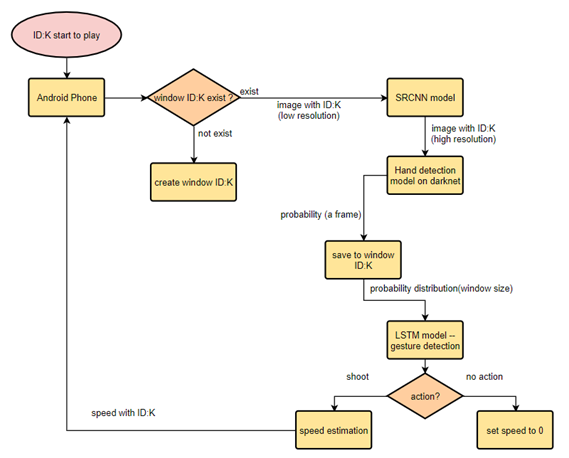
\includegraphics[width=10cm]{NN_SYS_structure.png}
    \caption{後端辨識系統架構圖}
    \label{fig:後端辨識系統架構圖}
\end{figure}

\subsubsection{SRCNN網路結構}
此處利用CNN神經網路將低解析度轉換為高解析度,以符合本地端訓練的照片高解析風格。以下呈現整體架構圖。

\begin{figure}[H]
    \centering
    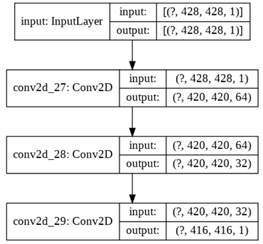
\includegraphics[width=6cm]{SRCNN_Structrue.png}
    \caption{SRCNN網路架構圖}
    \label{fig:SRCNN網路架構圖}
\end{figure}
\subsubsection{手部物件神經網路}

此專案是飛鏢遊戲,所以運算時間以及讀取時間需要降低,讓使用者不須等待就能得到射擊結果。
透過darknet平台,以yolov3為基礎更改其網路架構,以達成專屬類別輸出以及減少浮點運算次數的效果。並且,修改內部程式,達到傳輸效能提升,減少讀取時間。以下呈現經過多次實驗得到的新型網路架構。
\begin{figure}[H]
    \centering
    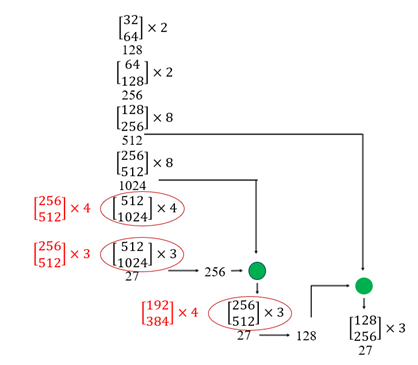
\includegraphics[width=8cm]{Darknet_Network.png}
    \caption{手部辨識神經網路架構圖(加速版)}
    \label{fig:手部辨識神經網路架構圖(加速版)}
\end{figure}



\subsubsection{LSTM神經網路}
手部物件辨識的機率分布存入window輸入至專門架設的LSTM網路結構中,並將輸出部份分為兩類別:無動作(0)、 射擊(1)。由於訓練資料的複雜度經過實驗後,發現並不需要使用更複雜的網路架構做學習,所以最終設計單層的LSTM。以下呈現LSTM網路架構。

\begin{figure}[H]
    \centering
    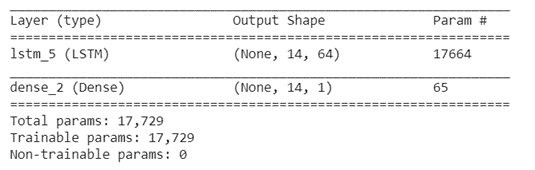
\includegraphics[width=8cm]{LSTM_Network.png}
    \caption{LSTM神經網路架構}
    \label{fig:LSTM神經網路架構}
\end{figure}


\subsection{神經網路實驗}

\subsubsection{優化darknet輸入評估實驗}

目的: 測試經過優化輸入後的darknet 與未優化輸入的darknet整體運作效能差距。
說明: 修改darknet中底層程式,並修改makefile後,重新編譯。讓darknet能加載numpy的內容,以及可以輸入陣列給darknet做偵測。而不需要再從硬碟讀取圖片作為輸入。
實驗方法:
\begin{itemize}
\item 實驗一未優化darknet輸入至原Yolo神經網路(未壓縮)做偵測。
\item 實驗二優化darknet輸入至原Yolo神經網路(未壓縮)做偵測。
\end{itemize}

測試方法:測試照片共100張的總時間,取平均時間。
\begin{figure}[H]
    \centering
    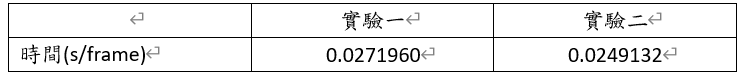
\includegraphics[width=10cm]{Darknet_Physics_Layer_OP.PNG}
    \caption{Darknet讀取優化比較}
    \label{fig:Darknet讀取優化比較}
\end{figure}
數據討論: 
每張降低0.00228秒,約 -8.4% 。	
結論: 
改採用優化darknet做為讀取輸入方式。


\subsubsection{神經網路手勢辨識實驗}

訓練資料生成:將訓練資料做resize成小圖片後再resize成原來大小。藉此產生訓練資料及測試資料。
訓練資料說明:兩張照片皆是由手機傳至伺服器後,重新resize成416*416大小(手部物件辨識網路輸入大小)。差別在於左側圖無經過SRCNN做高畫質轉換,而右側圖片有經過SRCNN做高畫質轉換。
將server照片經由SRCNN 轉換

\begin{figure}[H]
    \centering
    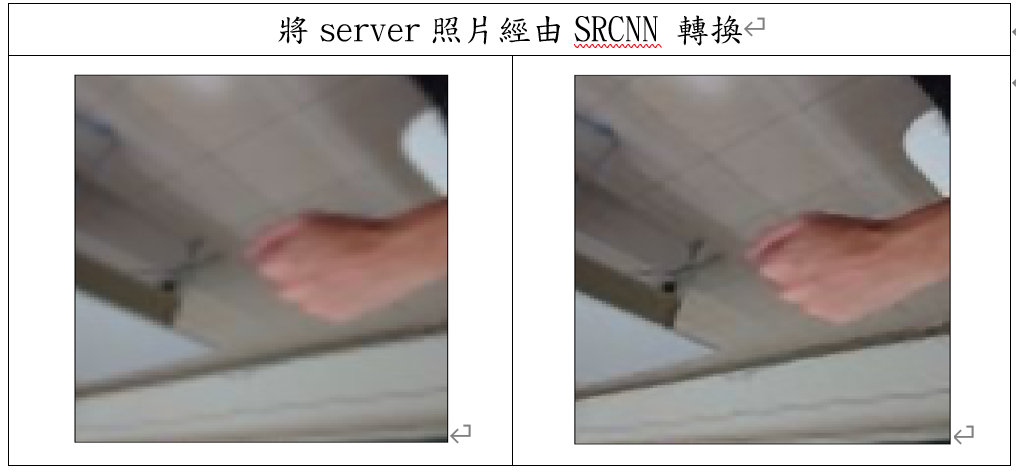
\includegraphics[width=10cm]{SRCNN_img.PNG}
    \caption{SRCNN效果圖呈現}
    \label{fig:SRCNN效果圖呈現}
\end{figure}

轉換結果評估:在未做SRCNN之前,手的輪廓並不明顯,影像顆粒度非常明顯。在做完SRCNN後,手的輪廓明顯從背景浮現,手上的陰影也更加明顯。

\subsubsection{未使用SRCNN測試結果}

\begin{figure}[H]
    \centering
    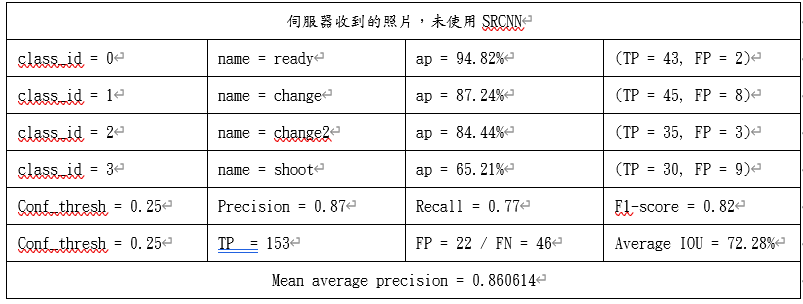
\includegraphics[width=10cm]{before_SRCNN_table.PNG}
    \caption{未使用SRCNN}
    \label{fig:未使用SRCNN}
\end{figure}

\subsubsection{使用SRCNN測試結果}

\begin{figure}[H]
    \centering
    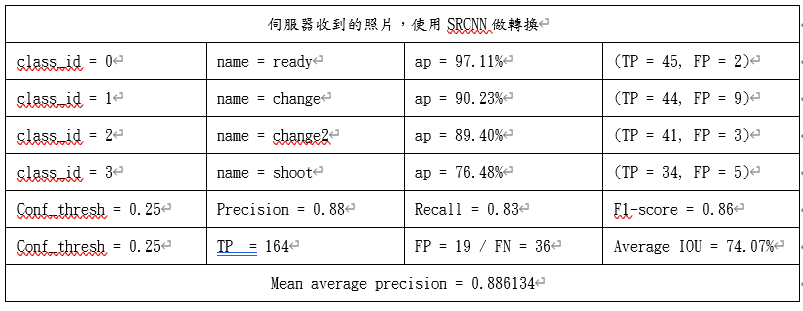
\includegraphics[width=10cm]{after_SRCNN_table.PNG}
    \caption{使用SRCNN}
    \label{fig:使用SRCNN}
\end{figure}

\begin{figure}[H]
    \centering
    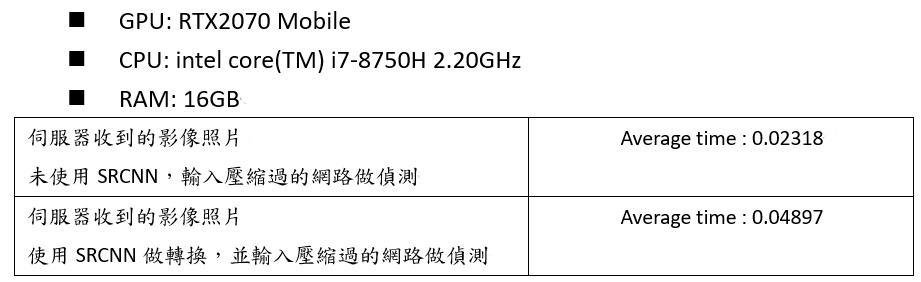
\includegraphics[width=10cm]{SRCNN_time.PNG}
    \caption{時間評估}
    \label{時間評估}
\end{figure}


評估:未做SRCNN之前,手的輪廓並不明顯,影像顆粒度非常明顯。做完SRCNN後,手的輪廓明顯從背景浮現,手上的陰影也更加明顯。使用SRCNN後mAP上升了2.5%。另外,做更深的細部分析。在最難判斷的類別id2、id3準確度皆有上升。推測可能是因為手的輪廓更明顯,從背景中凸顯出來,使手部物件辨識更加容易抓取手部位置,並更容易分類。另外,也沒有明顯的顆粒感在干擾CNN藉由filter擷取特徵的過程。
手部物件辨識:

\subsubsection{手部物件辨識網路訓練曲線圖}

\begin{figure}[H]
    \centering
    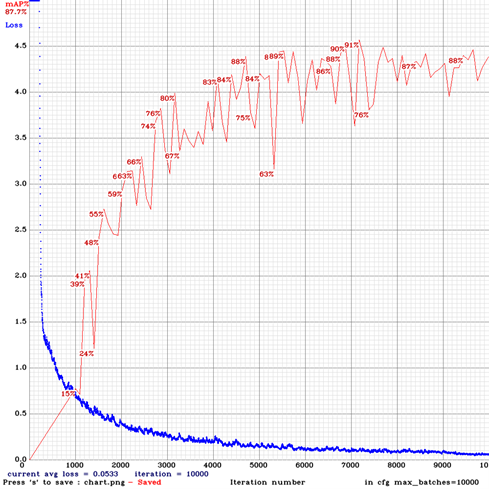
\includegraphics[width=10cm]{Darknet_Training_Curve_final.png}
    \caption{訓練曲線圖(Iteration)}
    \label{fig:訓練曲線圖(Iteration)}
\end{figure}

\begin{figure}[H]
    \centering
    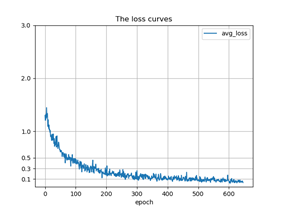
\includegraphics[width=10cm]{Darknet_Training_Curve2_final.png}
    \caption{訓練曲線圖(Epoch)}
    \label{fig:訓練曲線圖(Epoch)}
\end{figure}


觀察上方訓練結果,並沒有特別發現出現underfitting 或是 overfitting 的情形,雖然mAP以及loss在最後趨於穩定,表示其實learning rate 可以查是在做遞減,但是以整體訓練結果來看,validation data 測試所得的average mAP達到87.7%,表示訓練上收斂良好。

\subsubsection{新修改的CNN網路與原Yolo網路效能比較}

\begin{figure}[H]
    \centering
    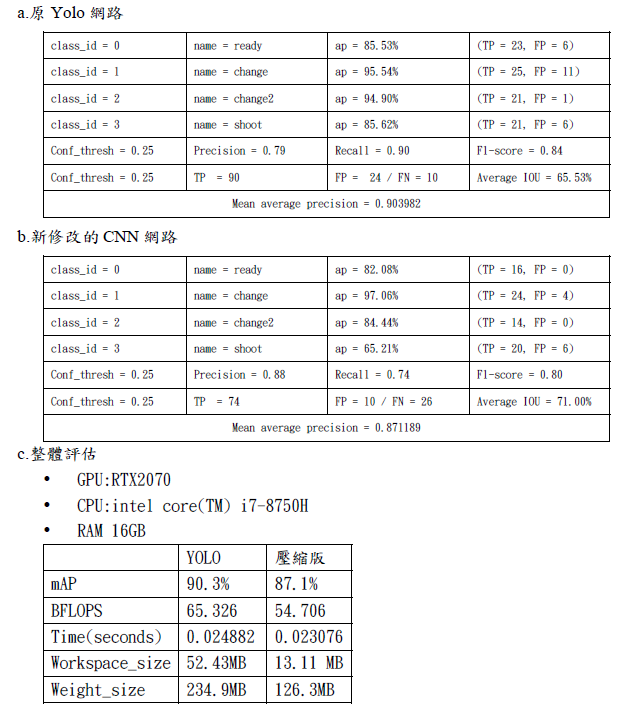
\includegraphics[width=15cm]{Darknet_Training_Table_final.PNG}
    \caption{}
    
\end{figure}




\subsubsection{window設計}

\begin{itemize}
\item X軸:單位時間
\item Y軸:次數
\end{itemize}

\begin{figure}[H]
    \centering
    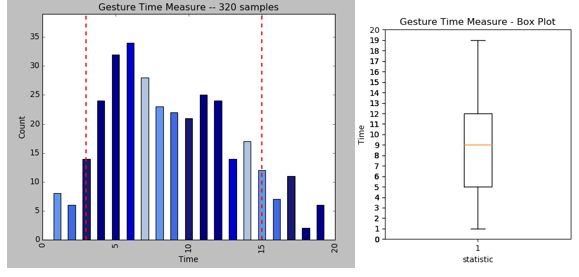
\includegraphics[width=10cm]{Windows_Size.PNG}
    \caption{}
\end{figure}

\subsubsection{LSTM網路設計實驗}

訓練資料生成:利用手部物件辨識得到的機率分布存成檔案,再將內部行數控制在window大小。由於資料不足,所以需要做資料擴充。利用random將機率做微調以及利用平移分布的方式,達到訓練資料擴充。
訓練資料共有500筆資料,切出200筆做為測試資料,評估模型。並將訓練資料由300筆增加至30000筆。

網路設計:
\begin{itemize}
\item 輸入維度  64 14 4
\item 將hidden state通過全連接層與sigmoid後輸出類別機率
\item 輸出機率0至1,threshold = 0.5,分為兩類發射(1)與無動作(0)
\item 學習率: Learning rate = 0.0001
\item 最佳化工具: Adam Optimizer
\item 損失函數: binary cross entropy
\item 未使用dropout
\item 訓練測試資料集比例0.8
\item 訓練次數100 epoch
\end{itemize}

\begin{figure}[H]
    \centering
    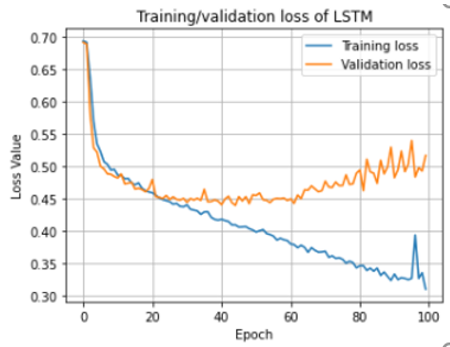
\includegraphics[width=10cm]{LSTM_Training_Curve.PNG}
    \caption{LSTM訓練曲線}
    \label{fig:LSTM訓練曲線}
\end{figure}

觀察上面Loss後,使用early stop技巧,將40 epoch 做為測試權重。
測試評估:使用真實資料100筆,各類別皆50筆,以避免資料分布不均導致評估不公正。

\begin{figure}[H]
    \centering
    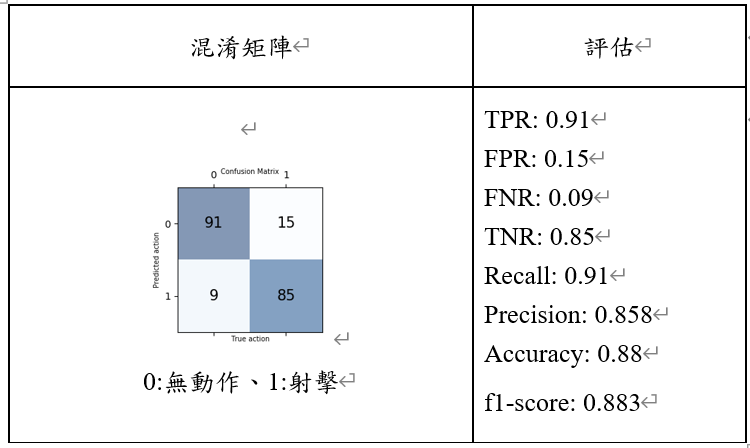
\includegraphics[width=10cm]{LSTM_Training_Table.PNG}
    \caption{手部辨識神經網路測試}
    \label{fig:手部辨識神經網路測試}
\end{figure}

分析:
由上面混淆矩陣,分類於第一類別(無動作)的正確率較高,而第二類別(射擊)的正確率相對較低。原因是,在製造第一類別(無動作)訓練資料時,可以將無動作訓練資料主要可以分為兩個類別,純粹無動作、或是有動作(但非射擊動作)。在第一部分純粹無動作是幾乎不會分類錯誤的,所以造成部份測試幾乎絕對正確。以至於第一類別(無動作)會正確率相較於第二類別(射擊)高。


\subsubsection{整體評估}
實驗方法:

使用200部影片,發射動作影片與無動作影片皆100部。給手部辨識神經網路辨識,辨識後根據該項實驗的設計來決定是否要傳送給SRCNN做高解析化,最後傳輸給LSTM網路做辨識。以LSTM網路辨識的準確度,以及整體辨識時間作為評估依據。

實驗設計:
\begin{itemize}
\item 實驗一:未優化darknet讀取影像照片方式
\item 未使用SRCNN + 未壓縮過後的手部辨識網路 + 單層LSTM輸出
\item 實驗二:優化darknet讀取影像照片方式
\item 未使用SRCNN + 未壓縮過後的手部辨識網路 + 單層LSTM輸出
\item 實驗三:優化darknet讀取影像照片方式
\item 未使用SRCNN + 壓縮過後的手部辨識網路 + 單層LSTM輸出
\item 實驗四:優化darknet讀取影像照片方式
\item 使用SRCNN + 壓縮過後的手部辨識網路 + 單層LSTM輸出
\end{itemize}

\begin{figure}[H]
    \centering
    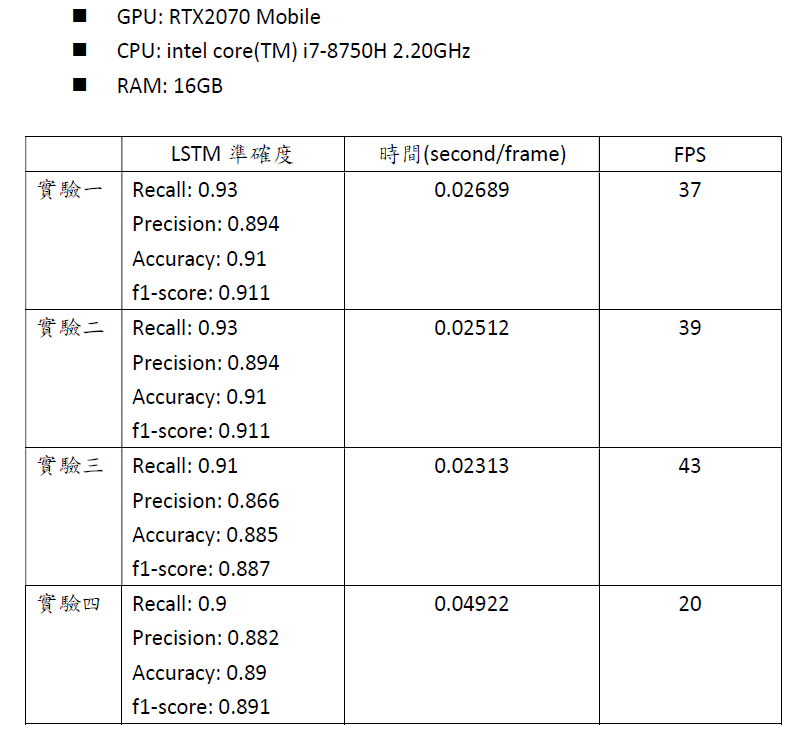
\includegraphics[width=10cm]{SUM_UP_EVAL.PNG}
    \caption{整體評估}
    \label{fig:整體評估}
\end{figure}


未壓縮優化的實驗一與加速優化的實驗三比較,FPS上升6。正確率卻只下降0.015。本專案在準確度達到一定要求下,會以縮短反應時間為主。因此選擇實驗三為本專題主要的偵測模式。
另外,對於額外使用SRCNN的實驗四來說,增加了高解析化後,雖然在(9)SRCNN實驗中顯示mAP上0.02,但是對於LSTM辨識結果並沒有太大作用,僅對於整體辨識結果正確率卻只上升0.05。而且辨識時間還增加一倍。因此往後的研究方向會以加速高解析化網路為主。

\begin{itemize}
\item 結論: 選擇實驗三作為目前專題的偵測模式。
\end{itemize}


% === Chapter ===
\chapter{討論&結論}
\section{討論}
\subsubsection{使用雲端運算架構原因探討}
在手機處理 AR 的應用已經較消耗手機資源的情況下,將神經網路的部分交由伺服器端運算,使用者的手機不需較高的配置,節省成本。另外,神經網路的運算本身就非常需要 GPU 的加速,即使手機有 GPU,但運算量遠小於伺服器的 GPU,因此為達到更佳的使用者體驗,也是放在雲端運算的原因之一。
當然在雲端運算架構也有缺點,若是使用者在離線的情形下,就無法遊玩此遊戲,不過在現在網路覆蓋率極高,相信在大部分的情況下,不會有這樣的情形發生。相對地,若伺服器端發生故障,則無法使用。
\subsubsection{物件較大影像的類別個數探討}
在網路深度較淺處,圖片較大,影像資源豐富,主要萃取low level的邊緣輪廓特偵,所以使用少量filter就可以完成。反之,深度較深時,經過多次pooling過程,影像大小變小,且影像資訊不斷被精餾萃取,需要使用更大量的filter萃取特偵。原本的Yolo是針對coco資料集做分類,分類數為80類別,所以在backbone的設計上,每層的filter需要更深、更大量。然而,在此專題中,雖然圖片模糊,但是只需要分為4類別,且物件偏大。因此,此實驗利用縮減backbone的方式來達到加速網路及減少浮點運算。越前層的low level feature map萃取的影像主要為基本線條元素,如果縮減破壞的話,對於後面feature map 的再萃取與one by one CONV的分類會影響很大。此專案所需分類數較少,只有4類別。因此,在medium 以及high level的feature map就不需要那麼多去描述紀錄最後要的特偵類別數。

\section{結論}
此系統主要透過 AR 以及神經網路的技術來模擬射飛鏢,首先用特徵點辨識,在實境影像上繪製虛擬標靶、虛擬飛鏢,再利用移動手機來決定飛鏢之方位,並使用手勢判斷發射的速度以及是否發射。手勢判斷是使用 UDP socket 來
手機後相機影像至伺服器端後,影像由佈署於伺服器端的神經網路模組SRCNN和LSTM 來辨識,再回傳飛鏢發射速度。發射過程中,透過世界
坐標系之轉換呈現在實境影像上。
未來希望能將以下幾點加入進模擬的考慮範圍當中,以模擬出更加符合真實狀況。
(1) 更精確的手勢辨識: 現在的樣本是基於組員們的手勢,而我們在運作過程發現仍會因為每個人的手部特徵不同,造成有少數幾位同學發射手勢,卻threashold過低,未來希望能將更多不同的手採納入訓練模型的樣本,更廣泛的辨識手勢。
(2) 手與鏢靶的深度關係: 因為現在所有的虛擬物件是貼在實景的上面,故手會被標靶遮擋,不符合實際狀況,未來希望透過 Computer Vision 的技術,利用手部的顏色以及手部的形狀,將手部貼在影像的最前端,不再被標靶遮擋。
\end{document}
